\documentclass{beamer}
\usepackage{xcolor}
%\usepackage{fontspec}
%\setmainfont{Georgia}
%\usepackage[T1]{fontenc}
\usepackage{winfonts}
\usepackage[backend=bibtex]{biblatex}
\usepackage{verbatim}
\renewcommand{\sfdefault}{georgia}

\bibliography{report}

%%%%%%%%%%%%%%
% Soton colourscheme

%primary palette:           RED    GREEN  BLUE
\definecolor{sotonblu}{rgb}{.00392 .26275 .34902} % soton blue
\definecolor{sotongrn}{rgb}{.00000 .44706 .45882} % soton green
\definecolor{sotoncya}{rgb}{.03922 .58824 .66275} % soton cyan
\definecolor{sotongry}{rgb}{.19608 .23922 .26275} % soton grey
\definecolor{sotonbei}{rgb}{.59216 .61961 .27059} % soton beige
\definecolor{sotonmet}{rgb}{.73333 .73333 .73333} % soton metal

%some secondary colors:
\definecolor{sotonyel}{rgb}{.99999 .70196 .00000} % soton yellow
\definecolor{sotonora}{rgb}{.99608 .24314 .07843} % soton orange
\definecolor{sotonred}{rgb}{.94118 .05882 .17255} % soton red
\definecolor{sotonrus}{rgb}{.67059 .07059 .06275} % soton russet
\definecolor{sotonbrn}{rgb}{.54118 .25490 .16863} % soton brown
\definecolor{sotonpnk}{rgb}{.88627 .41176 .62353} % soton pink
\definecolor{sotonppl}{rgb}{.32549 .12157 .26667} % soton purple


\setbeamertemplate{background canvas}[vertical shading][top=sotonblu,bottom=sotoncya]
\setbeamercolor{background canvas}{bg=}
\setbeamercolor{button border}{bg=sotonblu, fg=sotonblu}
\setbeamercolor{button}{bg=sotonblu, fg=DarkRed}

\setbeamercolor{frametitle}{fg=sotonyel}
\setbeamercolor{alerted text}{fg=sotonyel}
\setbeamercolor{normal text}{fg=white}
\setbeamercolor{titlelike}{fg=sotonyel}
\setbeamercolor{author}{fg=white}
\setbeamercolor{date}{fg=white}
\setbeamercolor{item}{fg=white}

%%%%%%%%%%%%%%%%%%%%

\title{Why Julia?}
\author{Jonathon Waters}
\institute{
	Cohort 1,\\
	EPSRC CDT in Next Generational Computational Modelling,\\
	University of Southampton
}
\date{}

\begin{document}
\frame{\titlepage

\includegraphics[height=1cm]{Images/sponsor-wo}\hfill
\includegraphics[height=1cm]{Images/uos_grey_large}}

\setbeamertemplate{headline}{
	\vskip25pt % horizontal line
	\vskip-21pt\hspace{2pt}\hfill
\includegraphics[height=7mm]{Images/sponsor-wo}\hspace{3.5mm}
\includegraphics[height=7mm]{Images/uos_grey_large}\hspace{3.5mm} % logo on the right
}

\setbeamertemplate{footline}{
	\vskip-8pt % horizontal line
	\hspace{12cm} \insertframenumber/\inserttotalframenumber
	\vskip4pt
}

\begin{frame}
	\frametitle{Outline of Today's Talk}
	\begin{itemize}
		\item What is Julia?
		\begin{itemize}
			\item The Goals of Julia
		\end{itemize}
		\item Key Features of Julia
		\begin{itemize}
			\item Multiple Dispatch
			\item Performance
			\item Built-in Package Manager
			\item Calls to Other Languages
			\item Parallelism
		\end{itemize}
		\item Competitors
		\item ...
	\end{itemize}
\end{frame}

\begin{frame}
	\frametitle{What is Julia?}
	From julialang.org: \newline

	\textit{``Julia is a high-level, high-performance dynamic programming language for technical computing, with syntax that is familiar to users of other technical computing environments.''}

	\vspace{5mm}\textit{``It provides a sophisticated compiler, distributed parallel execution, numerical accuracy, and an extensive mathematical function library.''}
\end{frame}

\begin{frame}
	\frametitle{The Goals of Julia}
	\begin{itemize}
		\item The \textit{speed} of compiled languages (C/C++ and Fortran) \newline
		\item The \textit{dynamism} of high-level languages (Ruby, Python) \newline
		\item The \textit{mathematical notations} of Matlab \newline
		\item The \textit{general usage} of Python \newline
		\item The \textit{statistical ease} of R
	\end{itemize}
\end{frame}

\begin{frame}
	\frametitle{Key Features of Julia}

	\begin{itemize}
		\item Multiple Dispatch \newline
		\item Performance \newline
		\item Built-in Package Manager \newline
		\item Calls to Other Languages \newline
		\item Parallelism \newline
		\item ...
	\end{itemize}
\end{frame}

\begin{frame}[fragile]
	\frametitle{Features: Multiple Dispatch}

	\textbf{Two function calls:} \newline

	\verb|my_func(x, 2)| \quad and \quad \verb|my_func(x, "cat")| \newline

	\begin{columns}
		\column[T]{6cm}
		\textbf{Single Dispatch} \newline

		In single dispatch languages like Python, the function calls dispatch to the \textbf{same function}.

		\column[T]{6cm}
		\textbf{Multiple Dispatch} \newline

		In multiple dispatch languages like Julia, these function calls may or may not dispatch to \textbf{different functions} depending on the \textbf{type at run-time}.
	\end{columns}
\end{frame}

\begin{frame}
	\frametitle{Features: Performance}

	\begin{itemize}
		\item Julia uses a \textbf{LLVM} to perform ``Just-In-Time'' (\textbf{JIT}) compiling of code. \newline

		\begin{itemize}
			\item C and Fortran compile into machine code then run the resulting exectutable. \newline

			\item Python interperets instructions into bytecode on the fly, allowing for compatibility accross multiple platforms. \newline

			\item Julia combines these approaches, interpreting the instructions then compiling them into the native machine code of the system on which it is running. \newline
		\end{itemize}

		\item This lets Julia approach and (sometimes) surpass C in speed while still looking like simple Python or Matlab code.
	\end{itemize}
\end{frame}

\begin{frame}
	\frametitle{Features: Performance}

	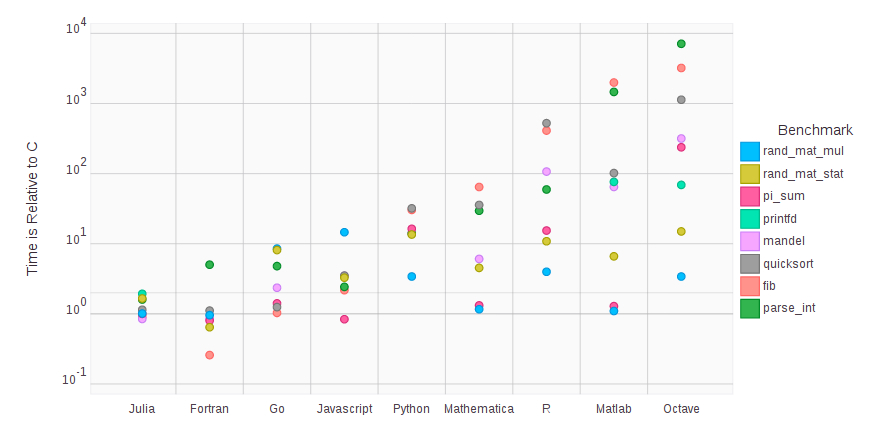
\includegraphics[width=11cm]{Images/perf1.jpg} \newline

	\small http://scienceblogs.com/catdynamics/2014/04/21/why-fortran-lives/
\end{frame}

\begin{frame}[fragile]
	\frametitle{Features: Performance}

	\small \begin{verbatim}
		# julia code for generating the mandelbrot set

		function mandelbrot(a)
		    z = 0
		    for i in 1:50
		        z = z^2 + a
		    end
		    return z
		end

		for y in 1.0:-0.05:-1.0
		    for x in 2.0:0.0315:0.5
		        if (abs(mandelbrot(complex(x,y))) < 2)
		            print("*")
		        else
		            print(" ")
		        end
		    end
		    println()
		end
	\end{verbatim}
\end{frame}

\begin{frame}
	\frametitle{Features: Packages}

	Julia features a built-in package manager: \newline

	\begin{itemize}
		\item Over 1100 registed packages (incl. Jupyter kernel). \newline

		\item No messing around with external package managers like pip or conda. \newline

		\item Interfaces to C, Fortran and Python (C++ being tested). Letting us reuse existing code wih little overhead. \newline

		\item Due to the compiler, packages have been developed quickly in pure Julia, allowing a phenomenal development speed.
	\end{itemize}
\end{frame}

\begin{frame}[fragile]
	\frametitle{Features: Parallelism}

	There are a number of methods of parallisation in Julia: \newline

	\begin{itemize}
		\item Remote Calls:

			\begin{verbatim}
				$ ./julia -p 2

				julia> r = remotecall(rand, 2, 2, 2)
				Future(2,1,3,Nullable{Any}())

				julia> s = @spawnat 2 1 + fetch(r)
				Future(2,1,6,Nullable{Any}())

				julia> fetch(s)
				2x2 Array{Float64,2}:
				 1.60401  1.50111
				 1.17457  1.15741
			\end{verbatim}
	\end{itemize}
\end{frame}

\begin{frame}[fragile]
	\frametitle{Features: Parallelism}

	There are a number of methods of parallisation in Julia: \newline

	\begin{itemize}
		\item Loop mapping:

			\begin{verbatim}
				$ ./julia -p 2

				a = SharedArray(Float64,10)
				@parallel for i in 1:10
				    a[i] = i
				end
			\end{verbatim}
	\end{itemize}
\end{frame}

\begin{frame}
	\frametitle{Thank You}
	\begin{center}
		Thank you all for listening and I welcome any questions. \newline

		Contact: J.M.Waters@soton.ac.uk
	\end{center}
\end{frame}
\end{document}
